\documentclass[12pt]{article}

\usepackage{hyperref}
\usepackage{amsmath}
\usepackage{enumitem}
\usepackage{graphicx}
\usepackage{eso-pic}
\usepackage{float}

\title{
\textbf{GuSynth: The Polyphonic Guitar Synth Pedal}\\
\vspace{0.5em}
\large System Overview and Design Description}


\author{Team 2: Kai, Zion, Barry, Nick, Yasmeen, Aaryan}

\begin{document}

\AddToShipoutPictureBG*{%
    \AtPageLowerLeft{%
        \hspace{1cm}% left margin from edge
        \raisebox{1cm}{% height from bottom
            
\includegraphics[width=10cm]{images/BE_Horizontal-Lockup_RGB_color.png}
        }
    }
}
\maketitle
\thispagestyle{empty}

\newpage
\tableofcontents  
\newpage

\newpage

\section*{Executive Summary}
This project explores the design of a guitar pedal that transforms traditional guitar sounds into tones resembling other instruments or synthesizers. Using a mixture of both analog and digital effects, this system aims to form a physical guitar pedal that combines multiple systems to achieve this. One of the biggest constraints to consider is latency; the system should produce the output sound fast enough to feel immediate during play.

\section{Introduction}
\subsection{Need and Goal Statements}
\textbf{Need Statement:} Guitarists want to be able to create the sound of another instrument without having to remove their guitar during live performance, or learn a new instrument.\\
\textbf{Goal Statement:} Allow guitarists to play the sounds of different instruments with their guitar in real time.

%old statements
%\textbf{Need Statement:} Existing guitar-controlled synthesizers cannot detect and play more than one note at once, which limits the expressiveness of the guitar.\\
%\textbf{Goal Statement:} Design a polyphonic guitar synth pedal that is intuitive for guitarists and suitable for live performance. 
%(ALLOW MUSICIANS TO PLAY DIFFERENT SOUNDS WITHOUT SWITCHING INSTRUMENTS IN REAL TIME (<10 ms))

\subsection{Design Objectives} %(Polyphonic is the objective/solution)

\begin{enumerate}[label=(\alph*)]

    \item \textbf{Polyphonic Note Detection} \\
    The guitar is inherently polyphonic, but accurate and general-purpose polyphonic note detection is still an open challenge. In order to provide accurate polyphonic note detection, the device needs to accurately infer the number of distinct notes played in a guitar chord, and their individual pitches.

    \item \textbf{Low Latency} \\
    A latency of $10\,\text{ms}$ is targeted, to facilitate an intuitive and enjoyable user experience. The player should not perceive any delay between playing a note and hearing the synthesized sound through their amplifier. This strict latency requirement drives many of our architectural and algorithmic decisions.

    \item \textbf{Form factor} \\
    The device must fit comfortably onto a guitar pedal board, and conform to the design language of existing guitar effects pedals. Additionally, the device must accept 9V DC power from a coaxial jack (5.5mm x 2.1mm, center-negative), standard for guitar pedals.

%    Note: By existing design language, I mean:\\
%    - Input goes from right to left \\
%    - Power jack is facing away from user \\
%    - All user controls located on the upward-face of the pedal\\
%    - Bypass footswitch is located on lower portion of the interface\\
%    - Knobs and parameter controls are located on the upper portion of the interface\\
%   Where should this information go?

\end{enumerate}

%\subsection{Existing Products}
% other guitar synth pedals (BOSS GT-3, 1997, has a monophonic guitar synth effect)
% melodyne and other software solutions (polyphonic detection)

\subsection{Target Audience (Personas)}
\begin{enumerate}[label=(\alph*)]
  \item \textbf{Bedroom Guitarist} \\
  A casual hobbyist looking to expand their creative palette without investing in additional instruments. They want expressive, unique sounds from gear they already own, in a package that is easy to set up and experiment with.
  \item \textbf{Recording Studio} \\
  A producer or session musician seeking precise, repeatable tones for tracking  and layering. They value low noise, consistent output, and seamless integration  into an existing signal chain or Digital Audio Workstation (DAW) workflow.
  \item \textbf{Live Performer} \\
  A performing musician who needs reliable, low-latency response under stage  conditions. They prioritize a rugged form factor, intuitive controls that can  be adjusted on the fly, and a sound that cuts through in a live mix.

\end{enumerate}

\clearpage
\section{Design of the Pedal}


\subsection*{Aesthetic Prototype}
\begin{figure}[H]
    \centering
    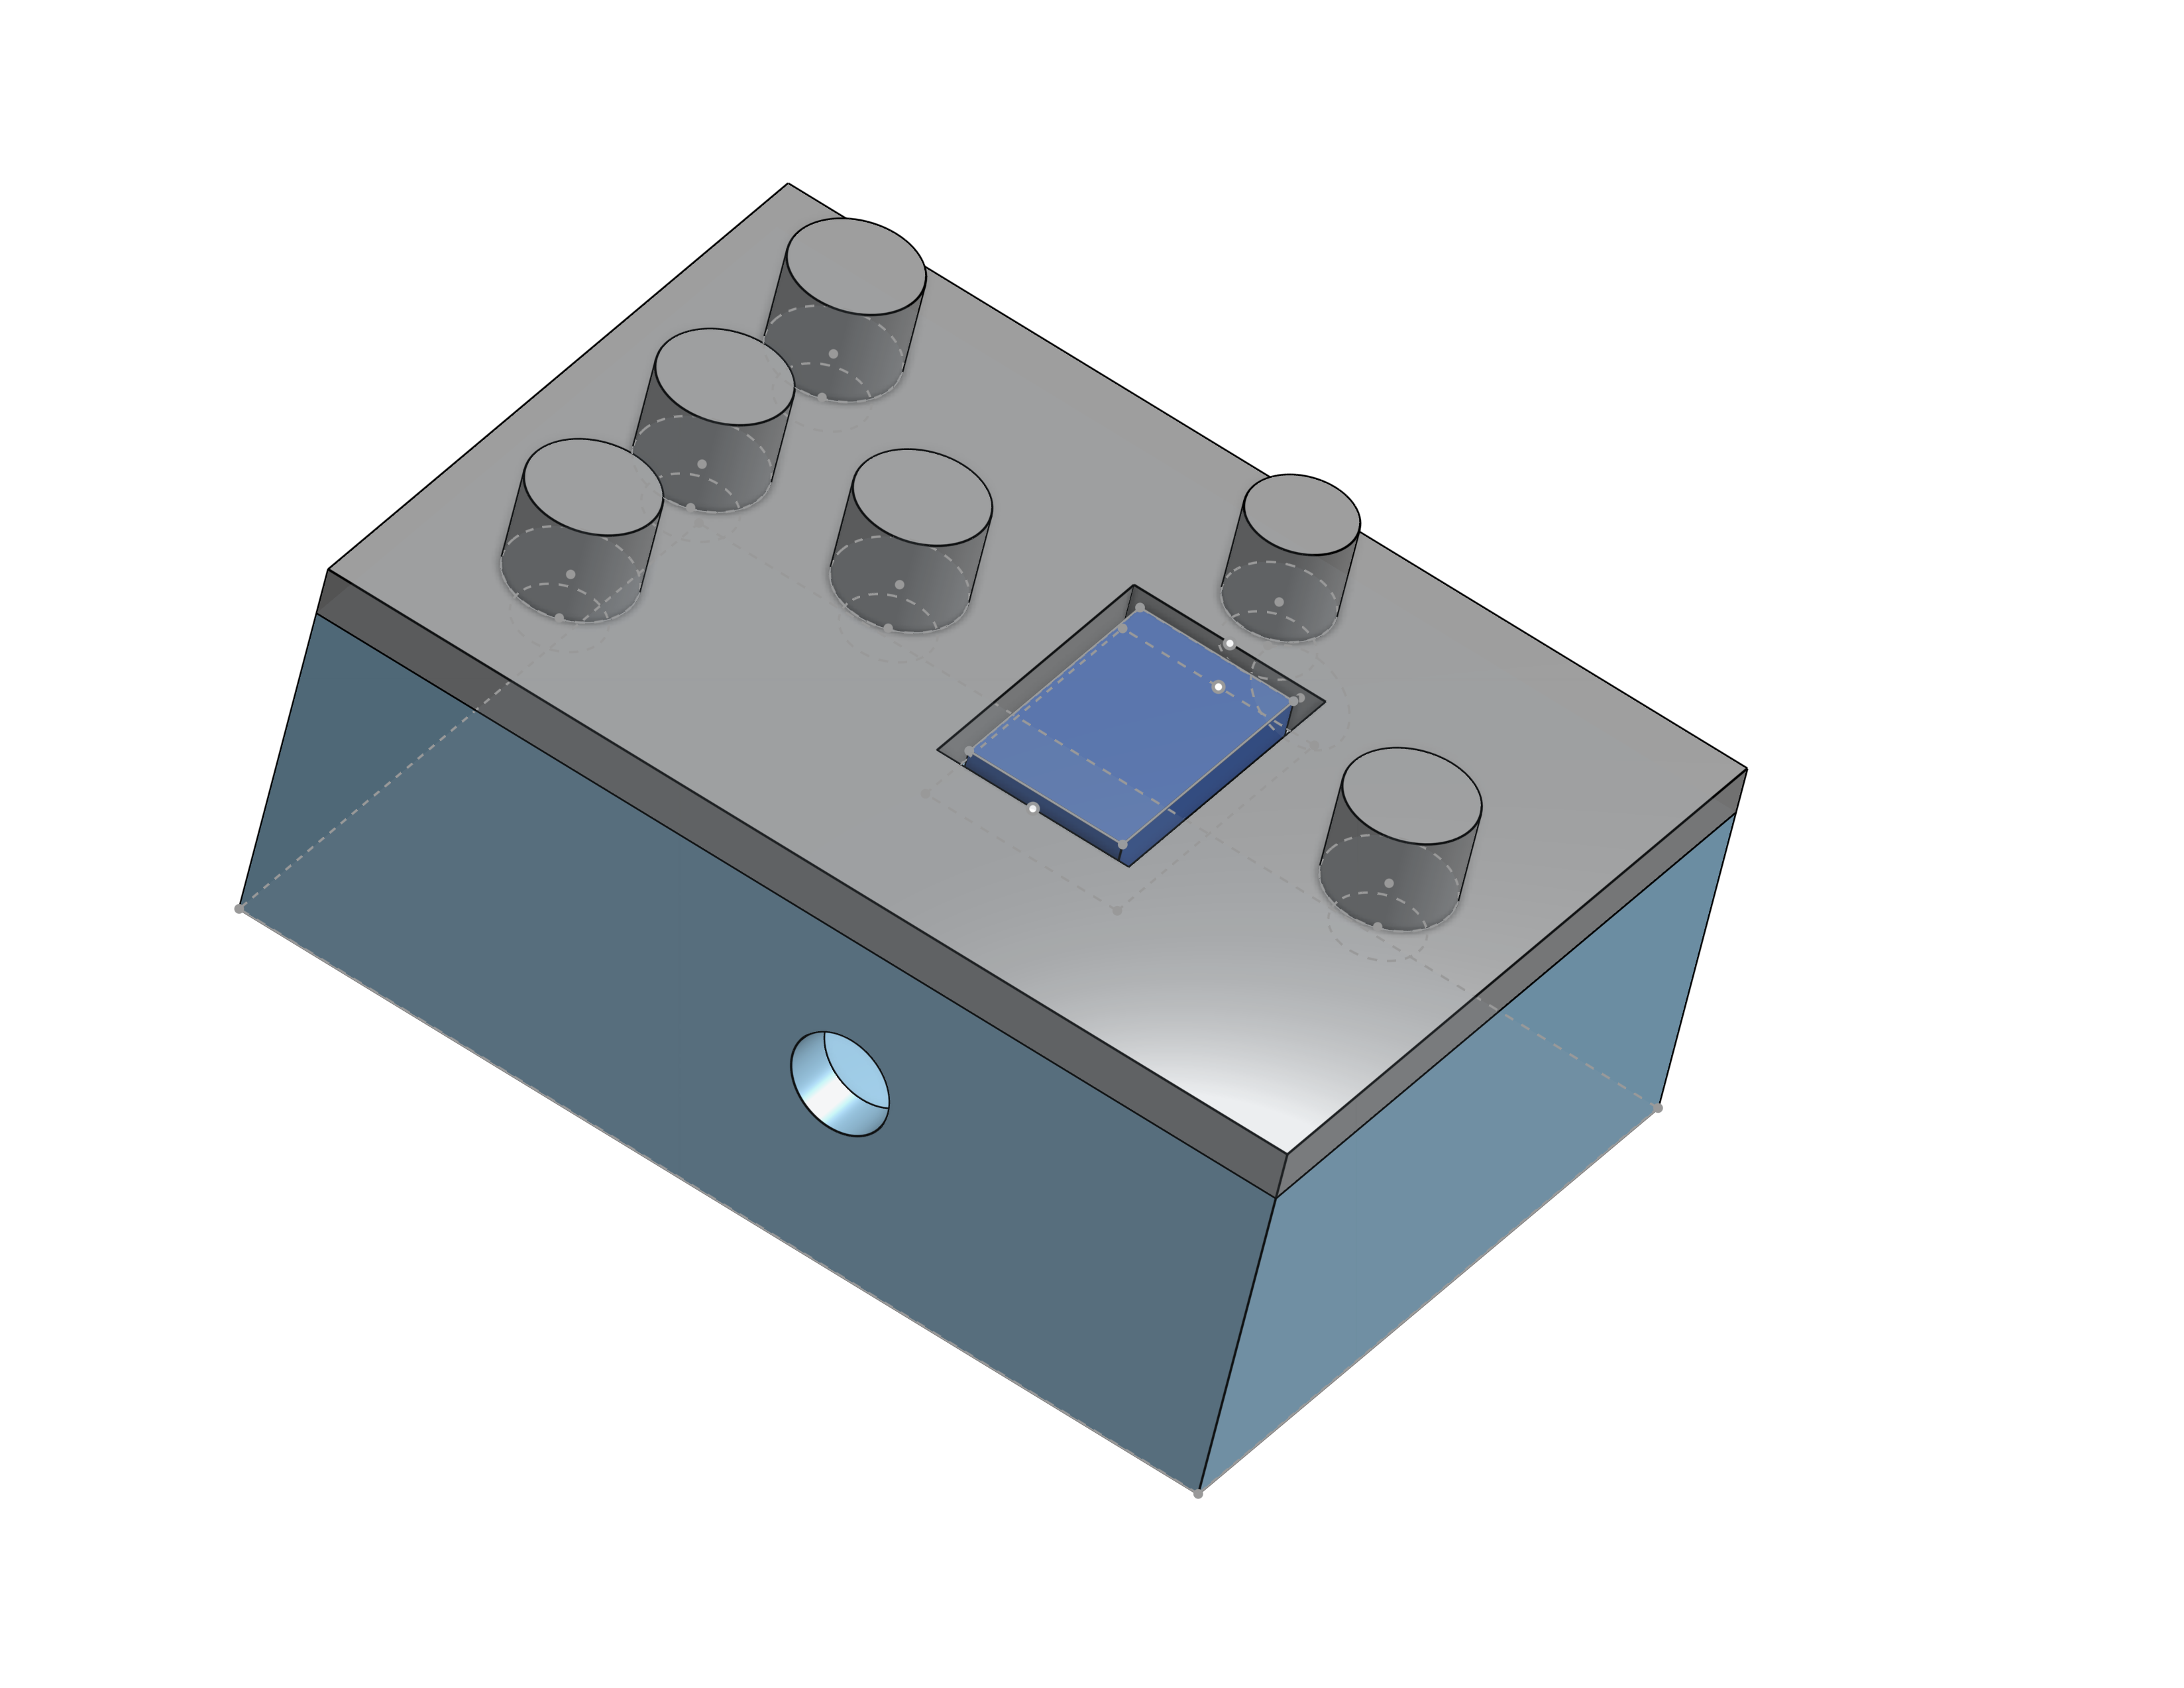
\includegraphics[width=1\linewidth]{images/pedalboxenclosureV2.png}
    \caption{Aesthetic Prototype}
    \label{fig:aesthetic-prototype}
\end{figure}


\subsection*{High-Level Block Diagrams}

\begin{figure}[H]
    \centering
    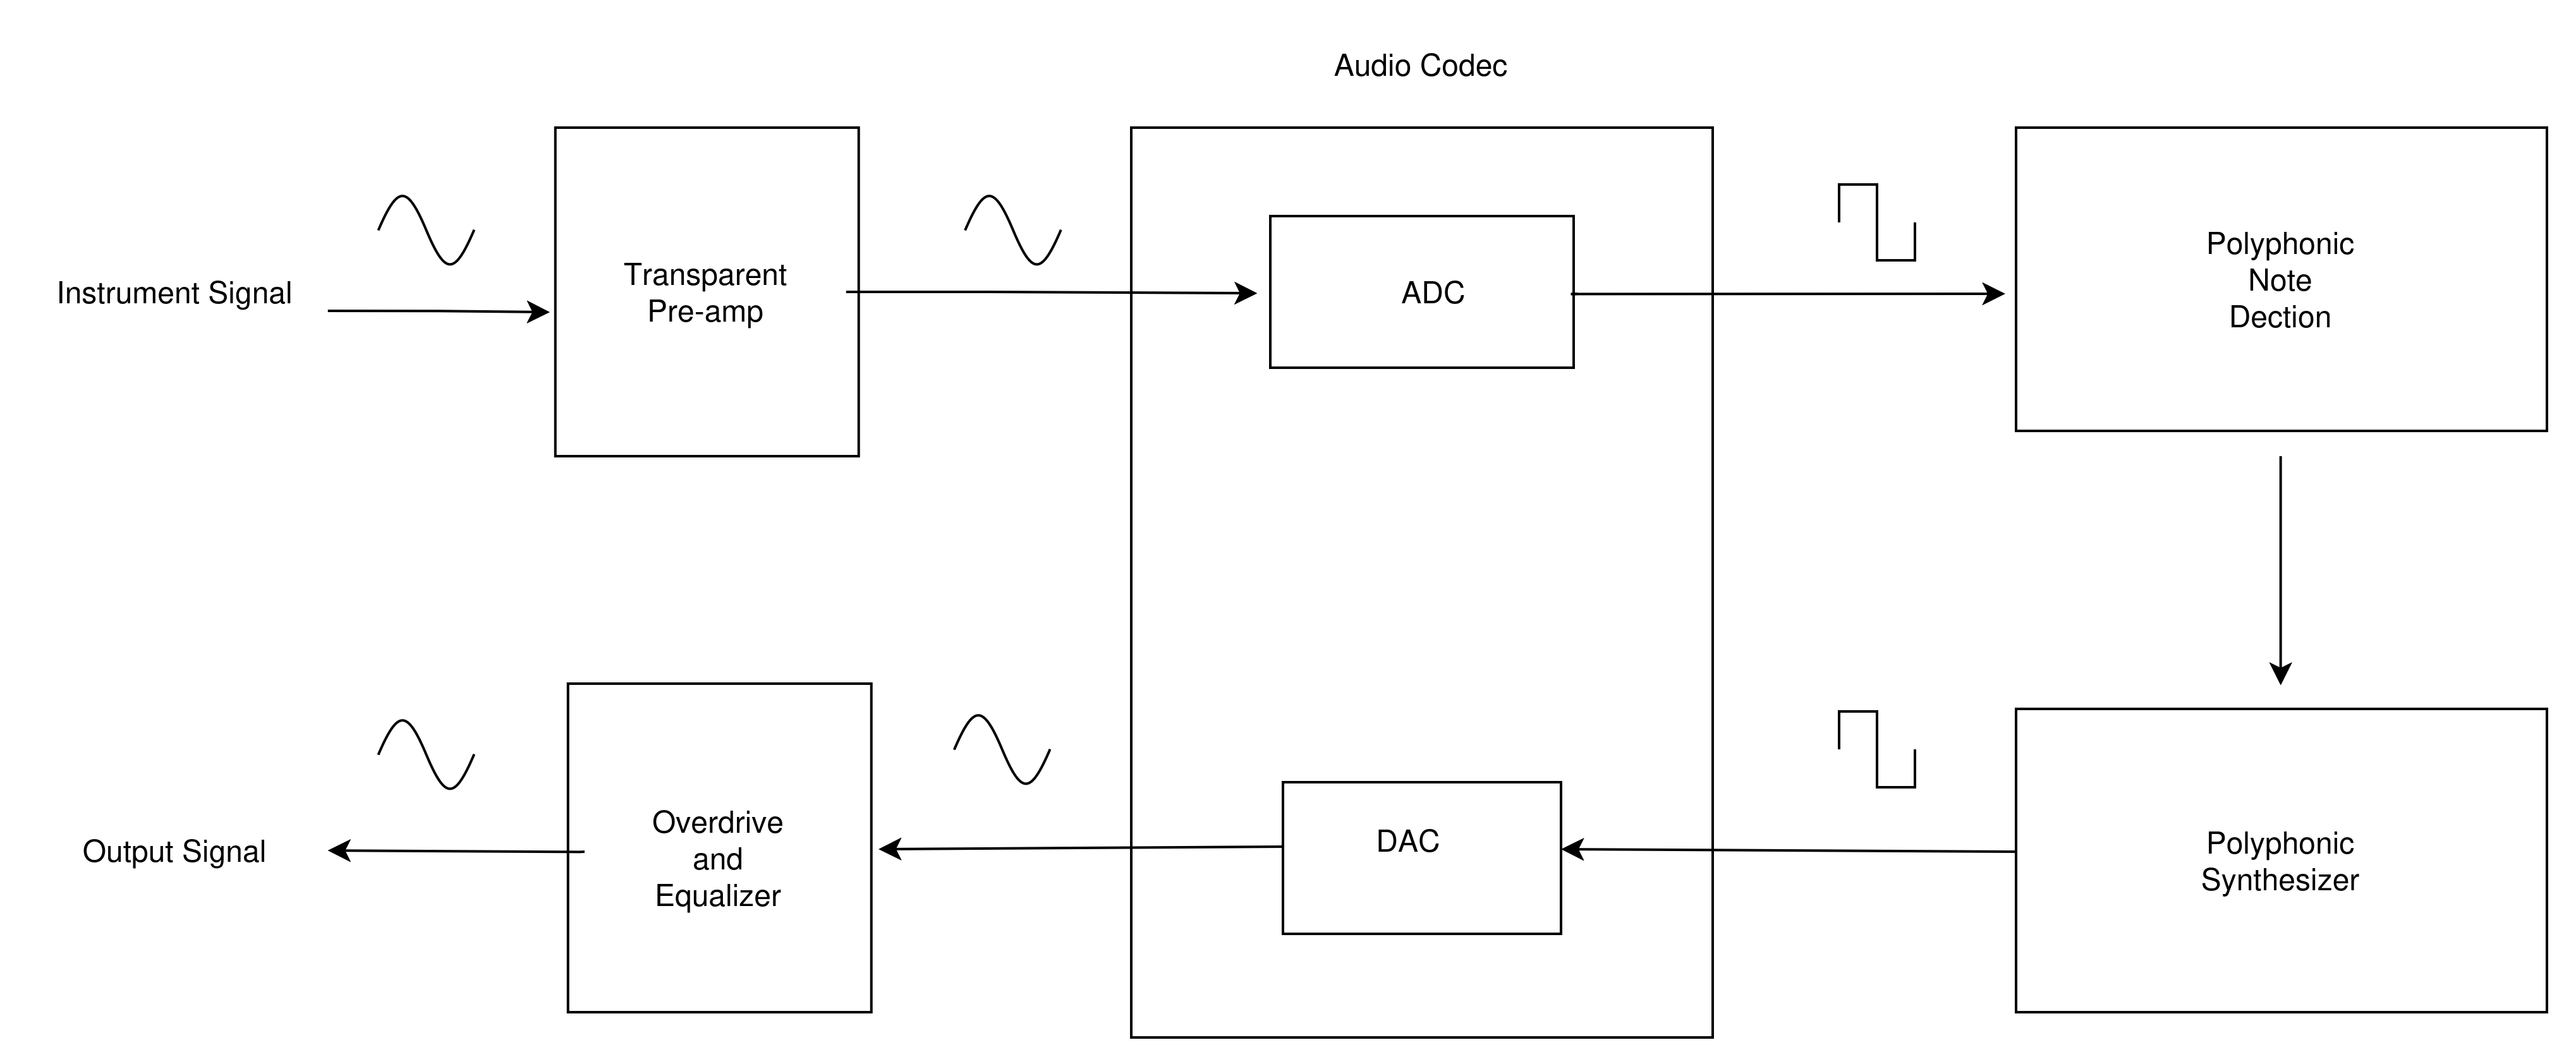
\includegraphics[width=0.9\linewidth]{images/audio_codec_diagram.png}
    \caption{Signal Path }
    \label{fig:block-diagram-signal}
\end{figure}


\begin{figure}[H]
    \centering
    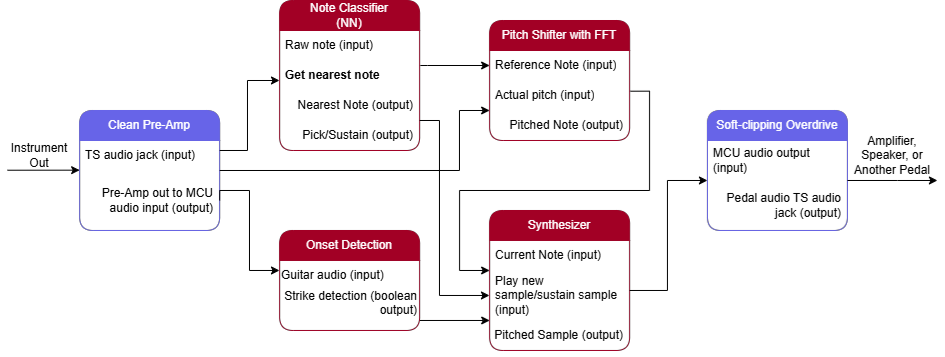
\includegraphics[width=0.9\linewidth]{images/schematic.drawio.png}
    \caption{Pedal Block Diagram}
    \label{fig:block-diagram}
\end{figure}

\subsection{Software System}

The software pipeline begins when the micro controller receives a digitized audio  stream from the analog-to-digital converter (ADC). The incoming samples are written into a ring buffer, which alternates between two fixed-size memory regions.  While one buffer accumulates new input samples, the other is made available for processing. This scheme ensures continuous, uninterrupted audio throughput and is  fundamental to meeting the low-latency requirements of the system.

Once a buffer is released for processing, the audio data is passed into a neural network inference pipeline. Rather than performing an explicit frequency decomposition,  the network approximates the pitch and onset characteristics of the incoming signal  directly, identifying which notes are present in the input. The microcontroller then uses these predictions to drive a synthesis engine, which generates an output waveform to produce the desired sound effect. The synthesized digital signal is subsequently converted back to an analog output via the digital-to-analog converter (DAC), where it is routed into the analog output stage.

\subsubsection{Neural Network}
A neural network is used to perform rapid note detection from the incoming guitar signal. Traditional pitch detection methods require observing multiple waveform periods, which introduces latency that is too high for a real-time pedal. Instead, a small neural network analyzes short audio windows (approximately 5–8 ms) to infer note identity directly from the signal’s transient and early harmonic content.
The model is implemented as a lightweight 1-D convolutional neural network designed for embedded inference. It predicts note class and onset information from each audio window, allowing the system to detect new notes almost immediately after a string is picked. These predictions provide an early estimate of the notes present in the signal, which can then be refined by later stages of the detection pipeline.

The trained network is exported to C and compiled directly into the microcontroller firmware, allowing it to run efficiently within the real-time audio processing loop. This approach enables low-latency note detection suitable for live instrument synthesis.
\subsubsection{Synthesizer}

The microcontroller supports any mathematically programmable audio effect, with the available effects limited only by the memory constraints of the hardware. Each effect is implemented as an independent processing function that transforms the incoming audio sample using a defined algorithm. The baseline implementation includes fuzz and distortion, which shape the waveform through non-linear gain functions. The firmware architecture allows developers to implement additional effects during the build phase, provided they can be expressed as a deterministic sample-by-sample transformation and fit within the available memory budget of the microcontroller. Once the effect is applied, the processed signal is passed through an automatic gain control (AGC) stage, which normalizes the output volume before the signal is forwarded to the DAC.

\subsection{Embedded Platform}
The embedded system bridges the digital and analog components of the pedal. The guitar signal from the transparent preamp enters an audio codec. The audio codec converts the analog waveform into discrete digital samples via an Analog-to-Digital converter. Then, these samples are transferred to the microcontroller using the Serial Audio Interface (SAI). Transferring the audio samples to the MCU is performed using Direct Memory Access (DMA). DMA places data into the MCU's RAM without CPU intervention, removing the need for the CPU to constantly poll and waste cycles. Once the samples are in RAM, the polyphonic and algorithms process the audio in software. When the signal has finished processing, it is sent back to the audio codec via DMA, then the Digital-to-Audio converter (DAC), and finally into the analog stage.

Audio is processed in small blocks to maintain our $<10\,\text{ms}$ latency target. Each stage in this pipeline is designed with real-time performance in mind. Furthermore, the pedal will feature a digital OLED screen. The screen indicates the current selected synth type. To change the currently selected synth and cycle through all options, a button is used. The OLED screen and the microcontroller communicate via the I2C protocol.

\subsection{Analog Circuits}
The pedal contains two primary analog circuits.

\subsubsection*{Transparent Preamp}
The preamp boosts the guitar signal to line level before feeding it into the ADC of the microcontroller. It is designed to be transparent so that the note detection neural network, which is trained on DI guitar audio, can work effectively.

\subsubsection*{Overdrive Circuit}

\begin{figure}[H]
    \centering
    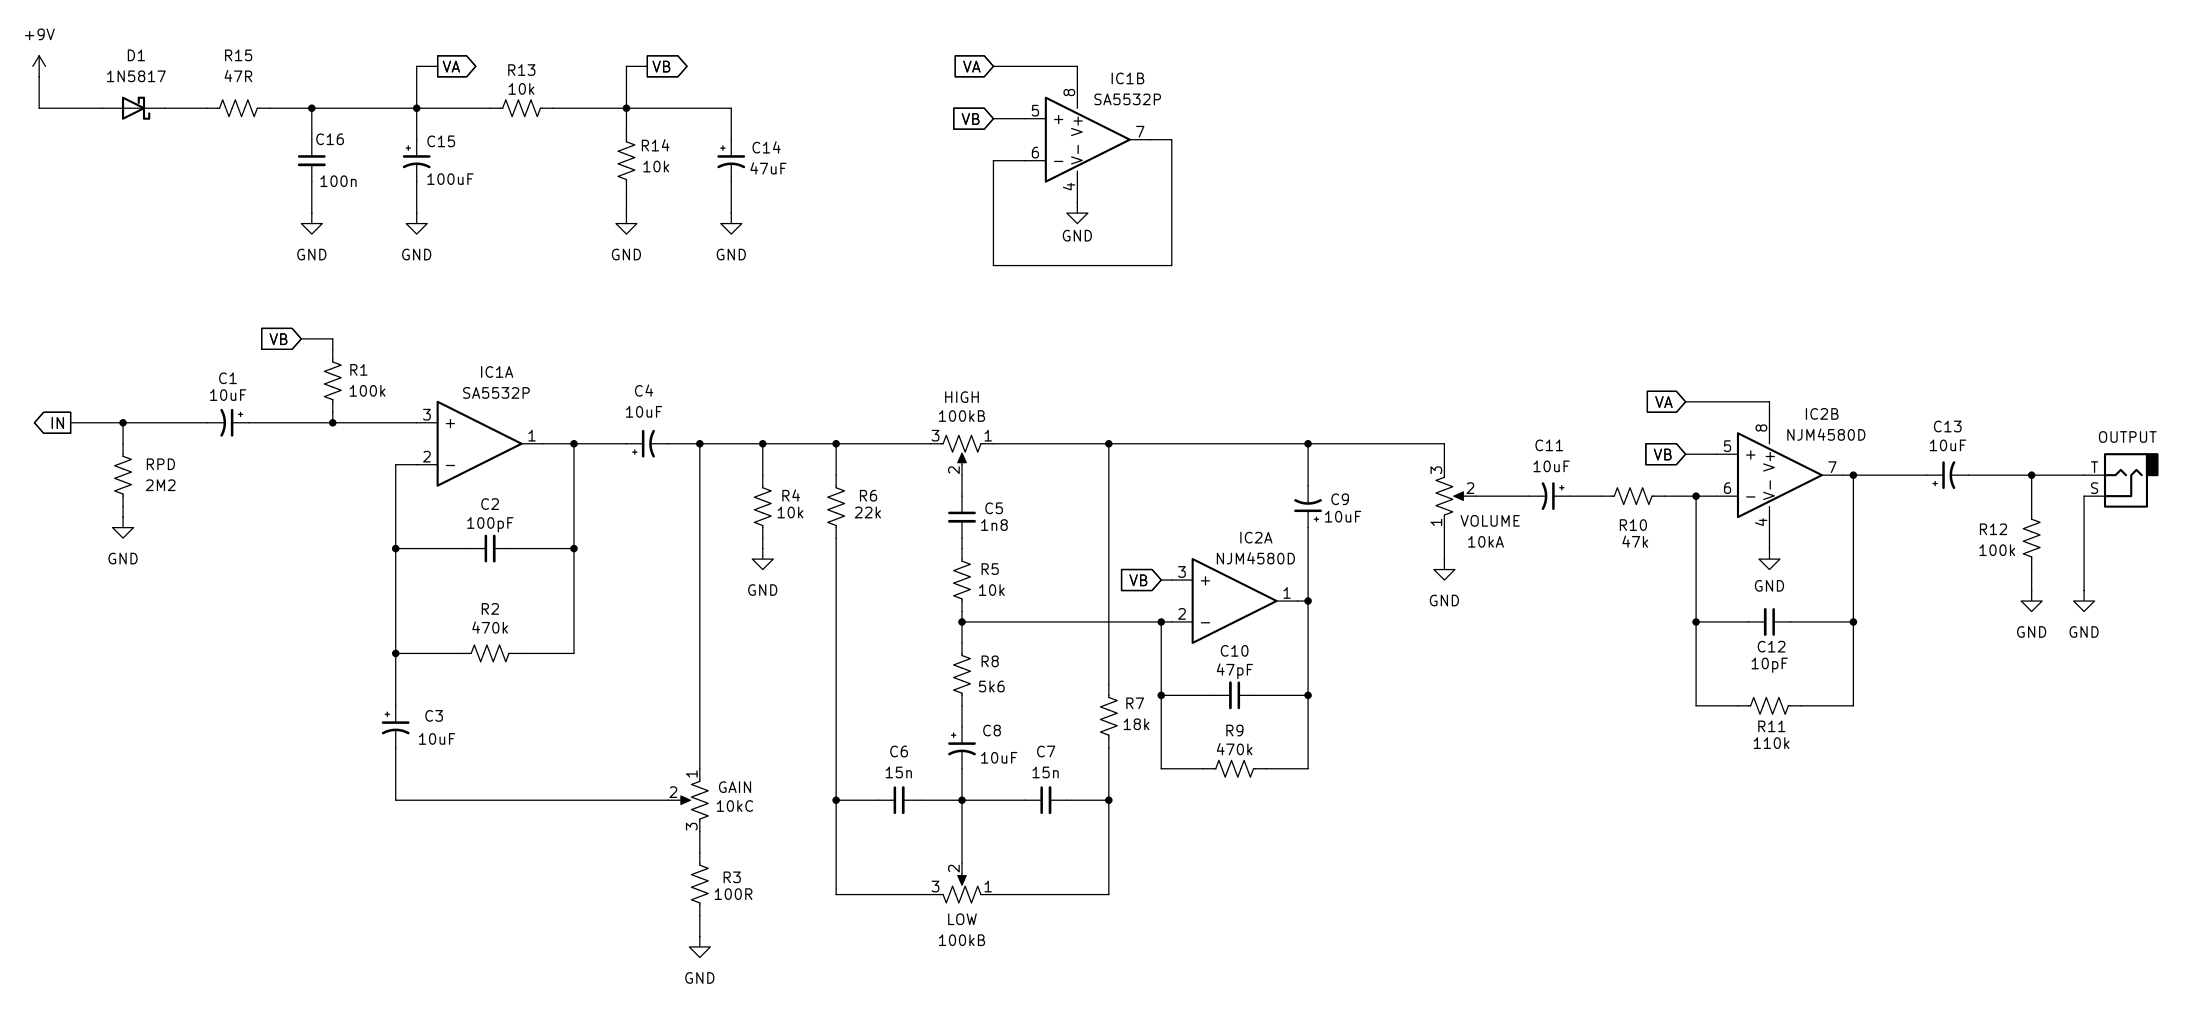
\includegraphics[width=1\linewidth]{images/424_schematic.png}
    \caption{Overdrive and Equalizer Circuit Schematic}
    \label{fig:424-schematic}
\end{figure}

The DAC of the microcontroller then feeds the synthesized audio signal into the second analog stage. This second stage is an overdrive circuit with EQ controls. This allows us to shape the tone and gain of the synth in the analog domain before sending it to the user’s amplifier, pedal chain, or other compatible equipment. This stage also provides master volume control.

Our current prototype draws inspiration from the Tascam 424 preamp architecture and a simple Wampler-style overdrive circuit. 

\subsection{Physical Construction}
The pedal enclosure follows the mechanical design conventions of standard guitar effects pedals in order to integrate easily into existing pedalboards.
The user interface consists of two rotary knobs, a push button for switching between synthesizer modes, and a foot-actuated bypass switch. The knobs are panel-mounted potentiometers connected to the microcontroller’s ADC inputs, allowing the user to adjust effect intensity and select different synthesis modes. The footswitch is designed for repeated mechanical stress during live performance.
A small OLED display is mounted on the top panel of the enclosure to provide feedback about the currently selected synthesizer mode. This allows the user to quickly verify which sound is active without relying solely on knob positions.
\section{Evaluation}
Evaluation of the pedal focuses on verifying that the system meets its functional requirements and performance goals. The evaluation process examines both hardware reliability and system performance, including power behavior, mechanical durability, and audio latency.

Testing procedures were designed to validate the pedal under realistic usage conditions similar to those encountered by musicians during rehearsal, recording, and live performance. These tests ensure that the device behaves predictably when subjected to typical physical interaction.

The evaluation phase also helps identify potential areas for improvement in the design, such as latency optimization, mechanical durability, or signal quality. By systematically verifying the core requirements of the system, we can properly determine that our prototype reaches our desired goals.
\subsection{Functional Prototype}

% Tests verify whether the design objectives are met
% Need to test every configuration
\subsection{Testing} 

\subsubsection{Power on}

\textit{Summary: The pedal should only power on when an input cable is connected. The power LED should only illuminate when the effect is not bypassed.}\\

Procedure:
\begin{enumerate}
    \item Initially, the pedal has no power or signal connections.
    \item Connect the pedal to a 9V DC, center-negative power supply.
    \item \textbf{Check}: The power LED should be off.
    \item Press the bypass switch.
    \item \textbf{Check}: The power LED should be off.
    \item Connect the output cable from the pedal to a powered-on guitar amplifier.
    \item \textbf{Check}: The power LED should be off.
    \item Connect the input cable.
    \item If the power LED is off, press the bypass switch.
    \item \textbf{Check}: The power LED should be illuminated, and the effect should be active.
    \item Disconnect the input cable.
    \item \textbf{Check}: The power LED should be off.
    \item Reconnect the input cable.
    \item \textbf{Check}: The power LED should be illuminated and the effect should be active.
    \item Press the bypass switch.
    \item \textbf{Check}: The power LED should be off and the unaltered guitar signal is passed to the amplifier.
\end{enumerate}
\subsubsection{Physical construction}

\textit{Summary: The pedal should support the full weight of an adult (max. 220lbs).}\\

Procedure:
\begin{enumerate}
    \item Place a flat, broad wooden platform onto the bypass switch.
    \item Load the platform with 220lbs of weight, taking care that it is supported entirely by the bypass switch.
    \item Remove the load, then the platform.
    \item \textbf{Check:} The pedal is not damaged or deformed in any way.
    \item \textbf{Check:} The bypass switch still toggles the effect.
\end{enumerate}

\subsubsection{Latency}
% This should be made more specific, and may need an illustration, but this is the idea.
\textit{Summary: The pedal must have a latency under 10ms.}\\\\
Equipment:
\begin{itemize}
    \item Oscilloscope
    \item Function generator
    \item 1/4" TS instrument cable x 2
    \item 1/4" TS jack, female x 2
\end{itemize}
Procedure:
\begin{enumerate}
    \item Configure the function generator to send a 440Hz, 100mVpp sinusoidal wave into a 1/4" TS jack.
    \item Channel 1 of the oscilloscope reads the output of the function generator from the 1/4" TS jack.
    \item A 1/4" instrument cable connects the output of the function generator to the input of the pedal.
    \item A 1/4" instrument cable connects the output of the pedal to the other 1/4" TS jack.
    \item Channel 2 of the oscilloscope reads the output of the pedal from the 1/4" TS jack.
    \item Configure the oscilloscope to simultaneously display Channel 1 and 2, with the same time scale.
    \item \textbf{Check:} Use cursors or other utilities on the oscilloscope to determine the phase shift of the waveform introduced by the pedal. If the pedal introduces a 10ms delay or higher, this test is failed.
\end{enumerate}

%------------------------------------------------
\section*{Appendix 1: Problem Formulation}
\subsection*{Conceptualizations}
The core concept of this project is a guitar pedal capable of transforming the sound of a guitar into the timbre of other instruments or synthesized sounds in real time. Unlike traditional guitar effects pedals that modify the waveform of the input signal directly, this system attempts to infer the musical notes being played and then generate a new signal based on those notes.

The final concept combines multiple techniques. A neural network is used to estimate note activity from very short audio windows, while a digital synthesis engine generates the output sound. Analog circuitry is used both before and after the digital processing stage to condition the signal and shape the tone.

This hybrid approach allows the system to maintain low latency while still enabling expressive sound transformations.
\subsection*{Brainstorming}
During the brainstorming phase, the team explored multiple possible features and system architectures for the pedal. Ideas included:

\begin{itemize}
\item Real-time instrument emulation (piano, strings, brass)
\item Guitar-to-MIDI conversion
\item Polyphonic pitch tracking
\item Neural network–based note detection
\item Analog distortion and tone shaping
\item Built-in effects such as fuzz or modulation
\item Visual feedback through an OLED display
\item Adjustable synthesis parameters through knobs
\item Pedalboard-compatible enclosure design
\end{itemize}

\subsection*{Decision Tables}
During the design process, several alternative approaches were evaluated. Table~\ref{tab:decision} summarizes the major design choices and the reasoning behind the final selections.

\begin{table}[H]
\centering
\resizebox{\textwidth}{!}{
\begin{tabular}{|l|l|l|l|l|}
\hline
Design Component & Option A & Option B & Option C & Selected Approach \\ \hline
Pitch Detection & FFT peak detection & Autocorrelation/YIN & Neural network & Neural network \\ \hline
Signal Processing & Fully analog & Hybrid analog/digital & Fully digital & Hybrid analog/digital \\ \hline
Synthesis Method & Sample playback & DSP synthesis & External MIDI synth & DSP synthesis \\ \hline
Display Interface & No display & LED indicators & OLED display & OLED display \\ \hline
Control Interface & Buttons only & Knobs only & Knobs + button & Knobs + button \\ \hline
\end{tabular}
}
\caption{Design decision comparison}
\label{tab:decision}
\end{table}
The neural network approach was selected because it offers the potential for lower latency detection compared to traditional pitch detection methods, particularly when analyzing short windows of audio.


\subsection*{Morphological Charts}
A morphological chart was used to explore combinations of possible subsystem implementations.

\begin{table}[H]
\centering
\begin{tabular}{|l|l|l|l|l|}
\hline
Component & A & B & C & Selected \\ \hline
Pitch Detect & FFT & YIN & NN & NN \\ \hline
Processing & Analog & Hybrid & Digital & Hybrid \\ \hline
Synthesis & Samples & DSP & MIDI & DSP \\ \hline
Display & None & LEDs & OLED & OLED \\ \hline
Controls & Buttons & Knobs & Knobs+Btn & Knobs+Btn \\ \hline
\end{tabular}
\caption{Design decision comparison}
\end{table}
%------------------------------------------------

\clearpage
\section*{Appendix 2: Planning}

\subsection*{Basic Plan / Gantt Chart}

\begin{figure}[H]
    \centering
    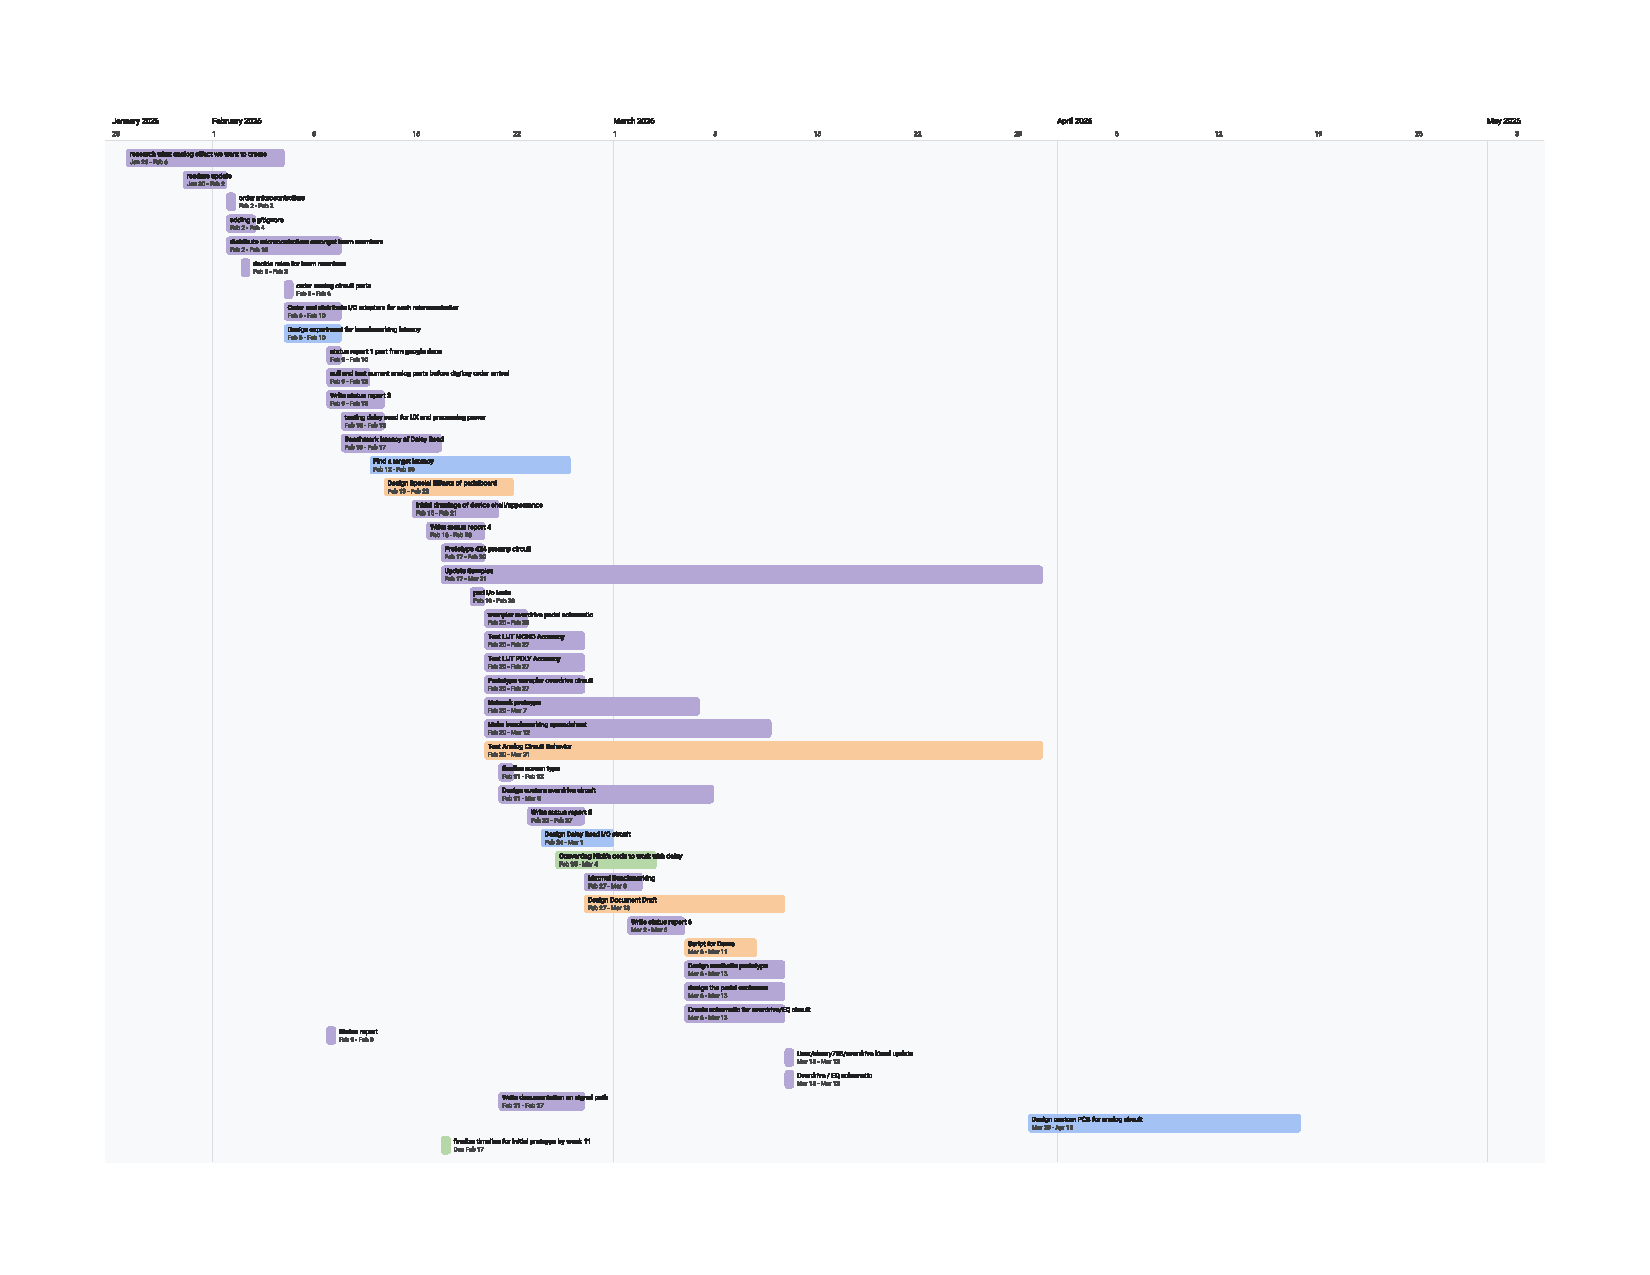
\includegraphics[width=1\linewidth]{images/ganttchart.pdf}
    \caption{Winter Quarter Gantt Chart}
    \label{fig:wintergantt}
\end{figure}


\subsection*{Division of labor during prototyping phase}
This graph is a screenshot from our GitHub Project of tasks assigned, in progress, on the backlog and completed grouped by our team members. The pink columns are what you're looking for, they are the completed tasks done by each member. 
Kai: Kaimul24
Nick: NickWeaver02
Aaryan: aaryanhlawat
Barry: sbarry753
Yasmeen: yamaniiiii
Zion: zion-silveyra
\begin{figure}[H]
    \centering
    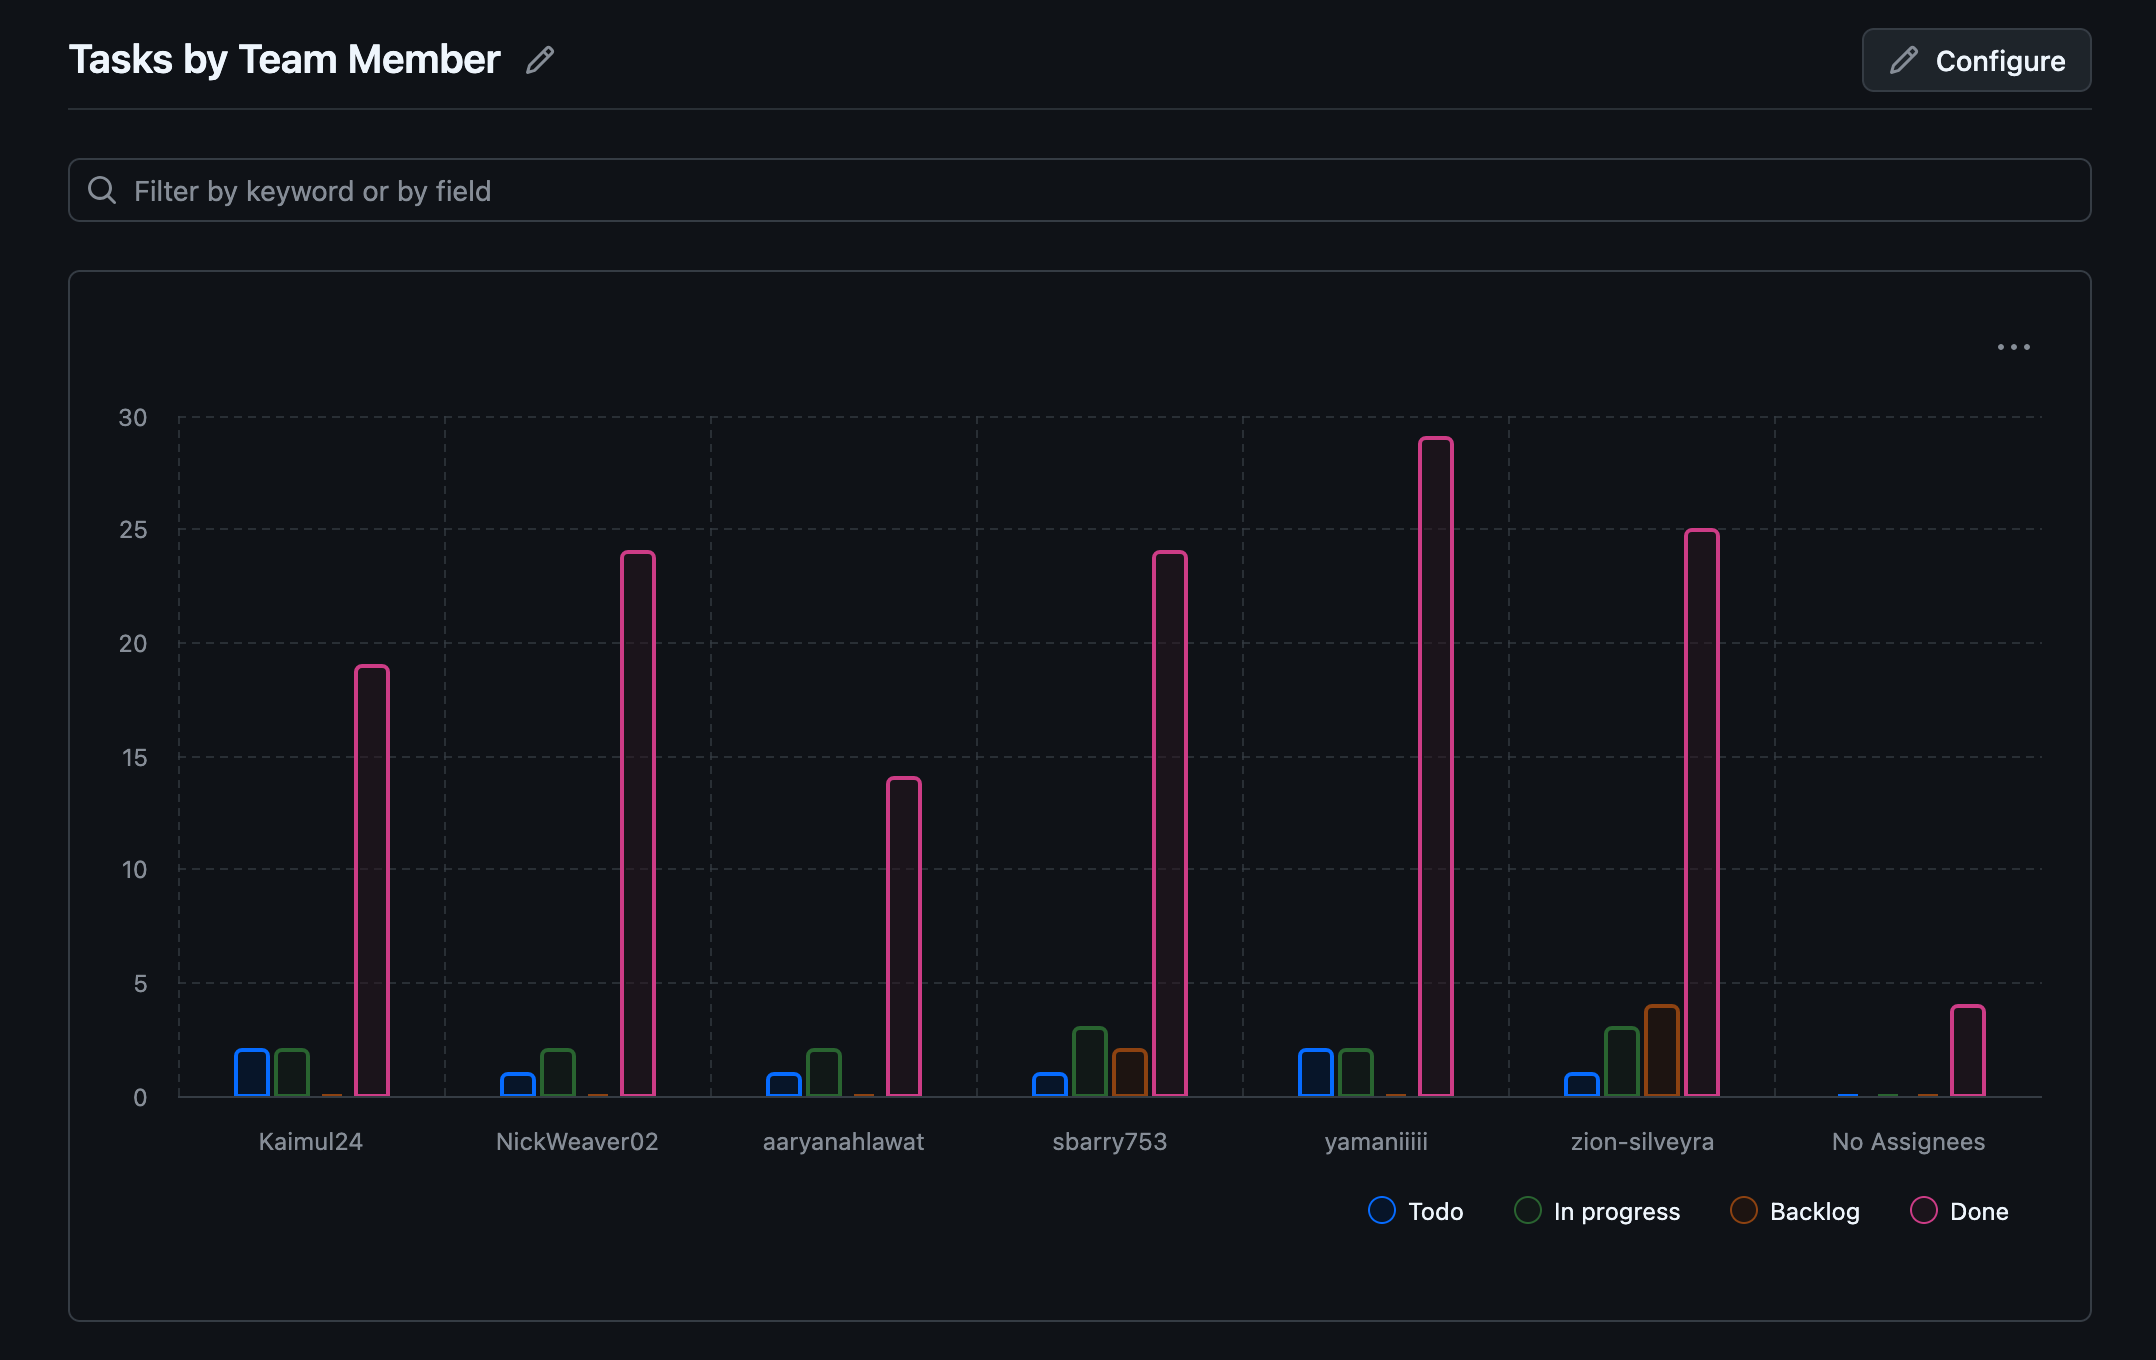
\includegraphics[width=1\linewidth]{images/Division of Labor update.png}
    \caption{Division of Labor}
    \label{fig:labor}
\end{figure}

\subsection*{Collaboration ( did you use tools beyond your repository? how did you assign tasks? )}
We use a GitHub Project that ties into our repository. There are a lot of tasks that are not necessarily able to be uploaded to a repository so we use the GitHub Project to track our members' progress on those.  

At the beginning, we used a Google Drive folder for collaboration on written assignments. We have since ported those documents to our repository, but we still use the Google Drive folder to organize collaborative files, like the Draw.io file for the overhead schematic, before pushing them to GitHub.

This design document is made with Overleaf, which is an online LaTeX editor that has collaborative functions like Google Docs. We then upload this work to our GitHub repository.

We communicate daily using our Discord server and have our discussions separated simply into a few channels: general, links and images, analog, embedded, and software. This helps us keep our communication organized and share our progress and findings.

We use Onshape, a collaborative cloud based CAD suite, to create our aesthetic prototype. There is a revision system included in Onshape. Our designs are then pushed to our GitHub repository.

We use Canva for making our demo slides. Canva is a collaborative cloud based graphic design suite that is easy to use. We push updated versions of our slides to our GitHub repository.


%------------------------------------------------
\section*{Appendix 3: Test Plan and Results}

\subsection*{Analog Effect Behavior}
We set out to make a distortion effect for the analog effect portion of the pedal. In order to test whether our distortion effect actually distorts the guitar signal we hooked up our circuit to an oscilloscope and a signal generator. The signal generator is generating a sine wave at 440Hz at 90mVpp to provide a clean A note from a guitar, the yellow wave. We're looking for the guitar's signal to clip at the peaks of the wave. The blue wave is the output from the distortion effect and it is clearly clipping the peaks of the signal and turning the guitar's sine wave into almost a pure square wave. This is the behavior of a hard clipping fuzz distortion effect which is the exact effect tested here.
\begin{figure}[H]
    \centering
    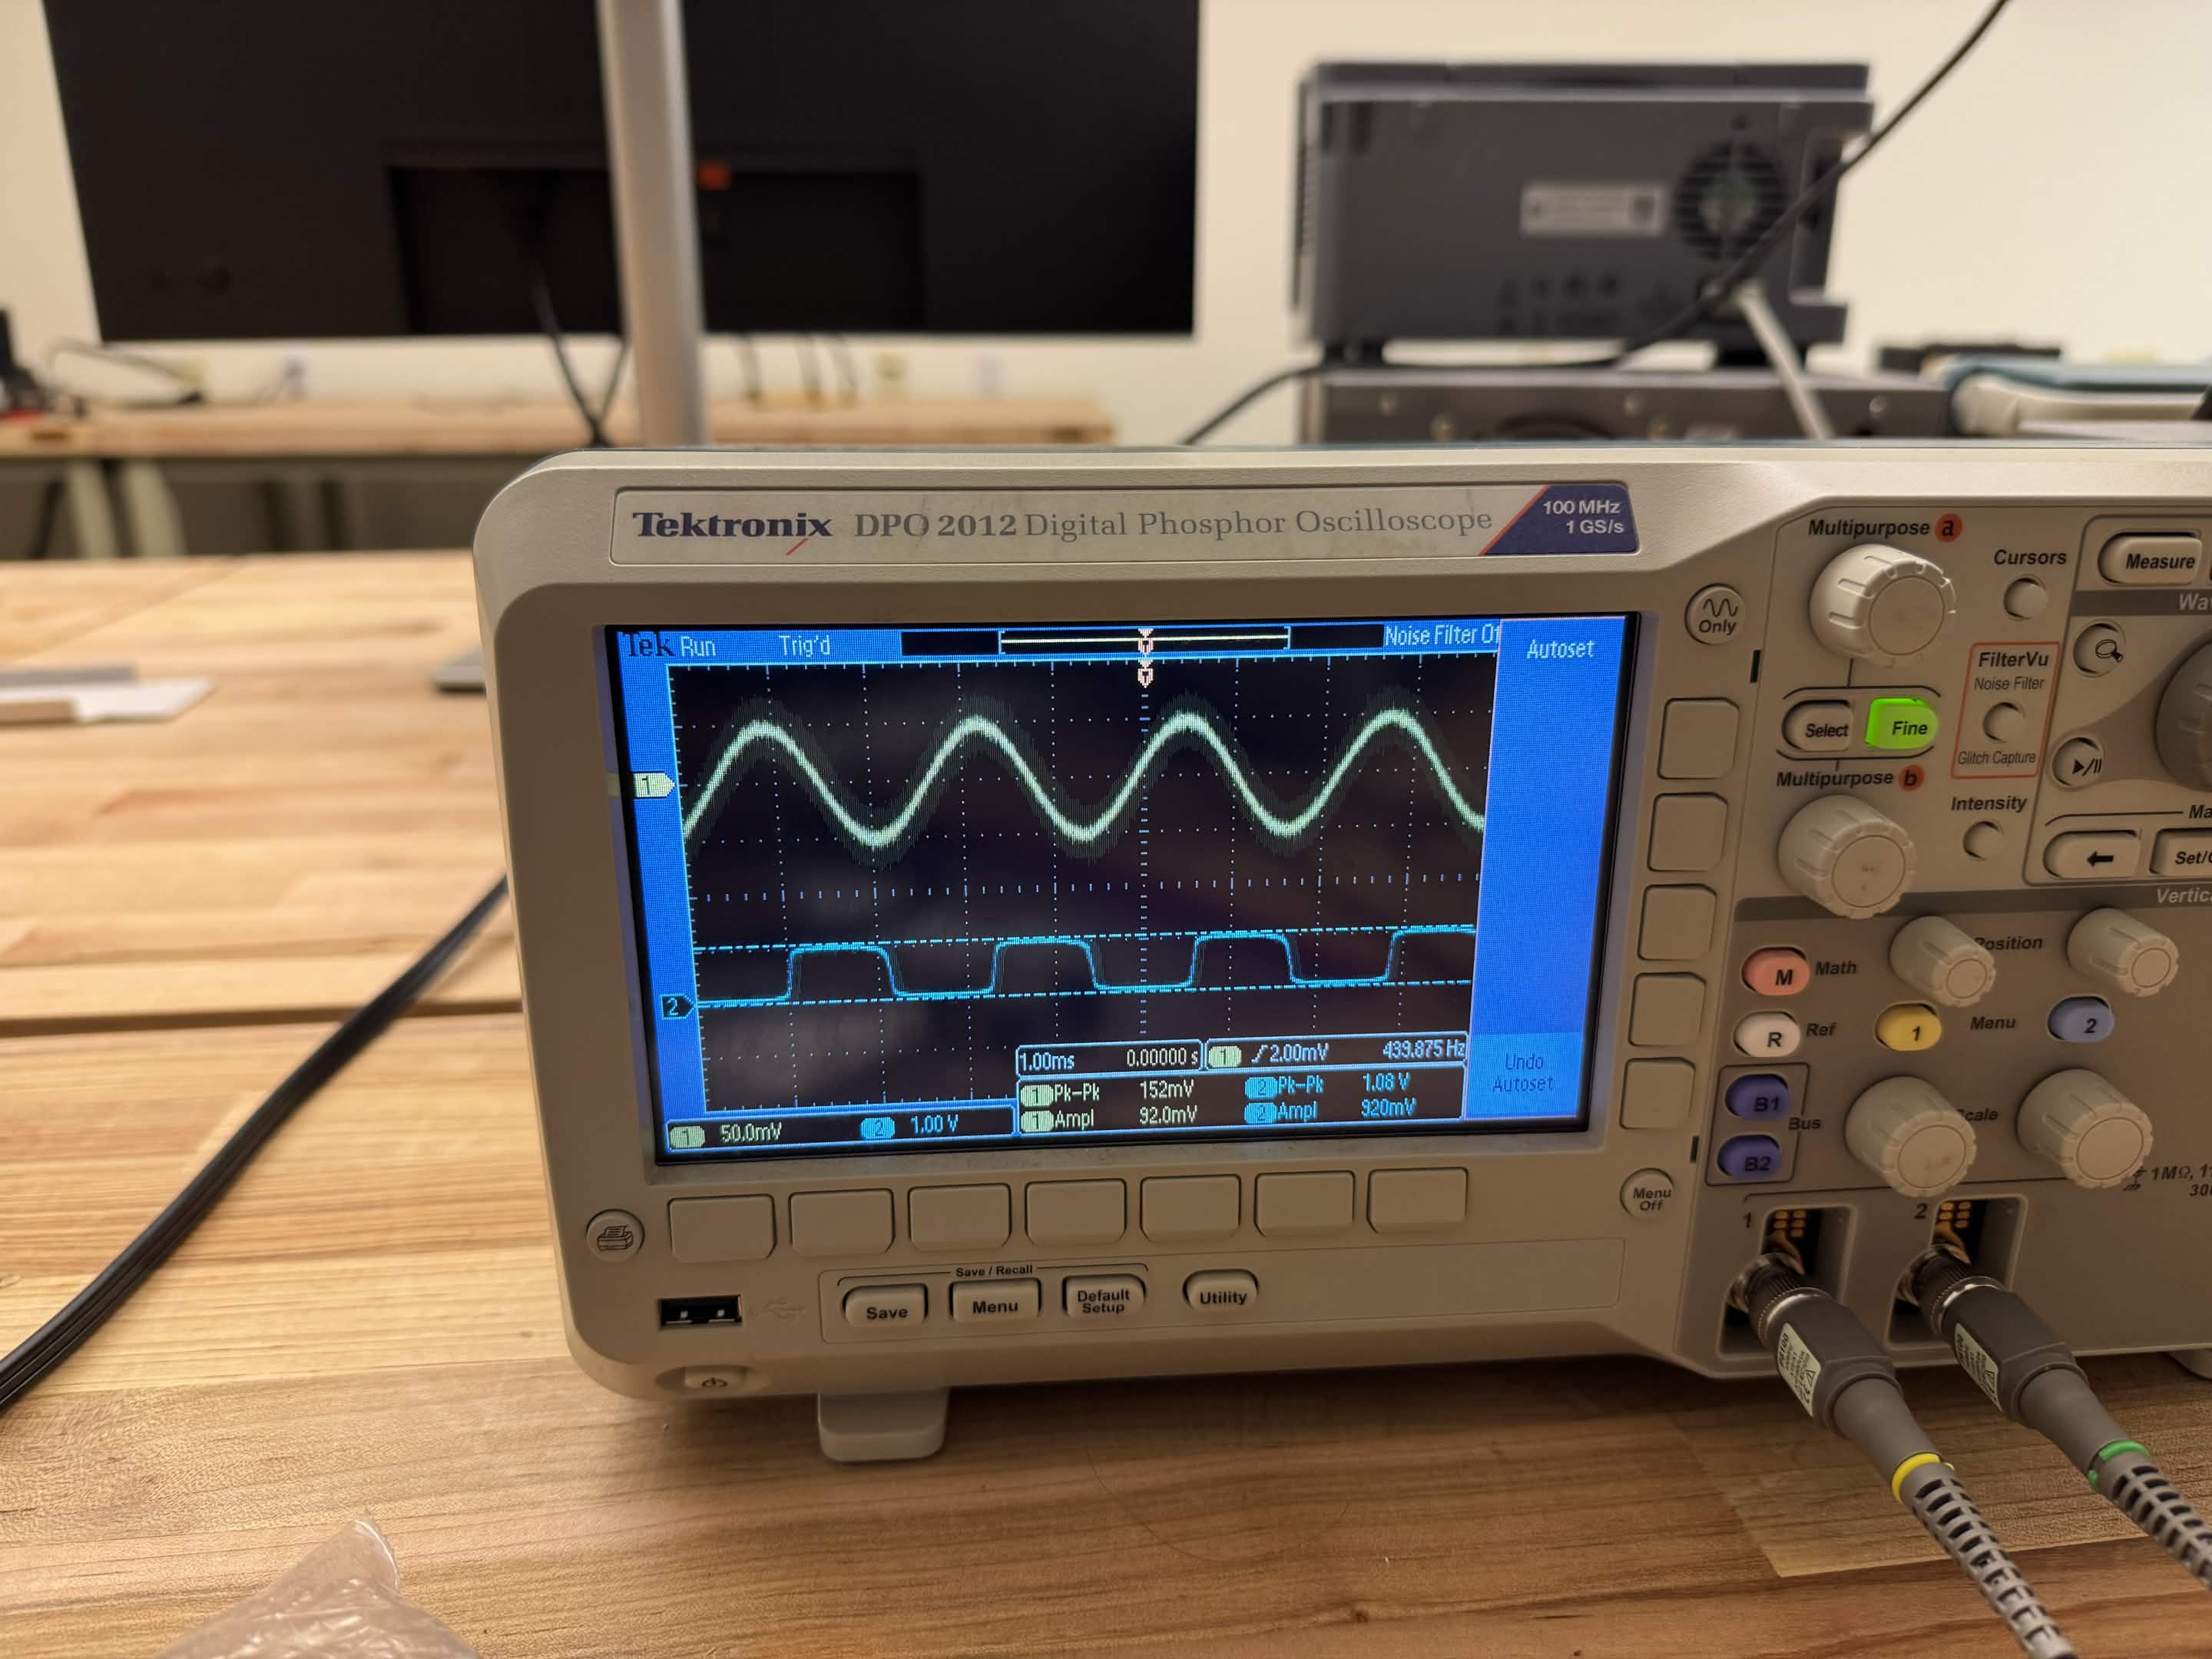
\includegraphics[width=1\linewidth]{images/analog-circuit-clipping.jpg}
    \caption{Clipping Distortion of an Analog Signal}
    \label{fig:analogclippig}
\end{figure}

\subsection*{Daisy Seed Benchmarking}
To get a sense of the processing power of the Daisy Seed (ARM Cortex M7 CPU), we decided to run a series of benchmarks. We first ran benchmarks for standard audio effects, similar to those found in the DaisyExamples repository provided by Electrosmith. In those tests, we determined that the actual audio effects did not result in any significant CPU load within a time budget. Then, we decided to stress test the MCU with matrix multiplication. This was an important benchmark to run because it is computationally demanding and relates directly to neural network inference performance. However, we found the MCU performed relatively poor in matrix multiplication, unaligned with real-time inference in mind. The MCU hit its maximum CPU load quickly during matrix multiplication, despite optimizations.

More detailed benchmarking information can be found in the \textit{Benchmarking} directory of our repository.

\begin{figure}[H]
    \centering
    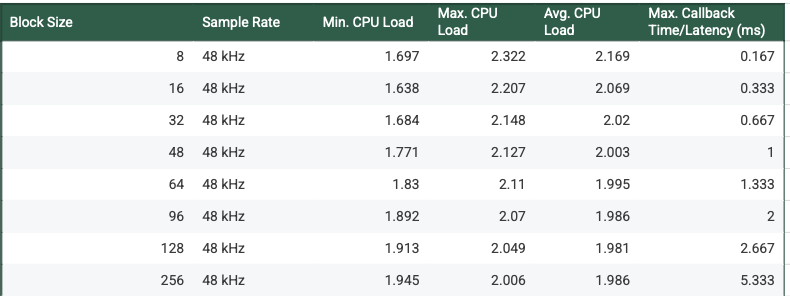
\includegraphics[width=1\linewidth]{images/benchmarktable.png}
    \caption{Benchmark Table (Passthrough)}
    \label{fig:benchmarkchart}
\end{figure}

\begin{figure}
    \centering
    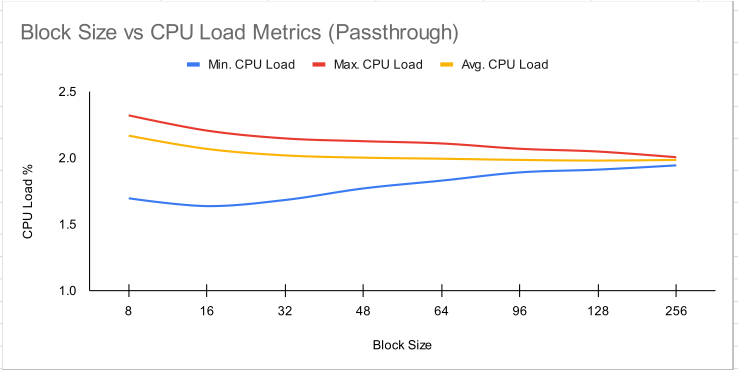
\includegraphics[width=1\linewidth]{images/benchmarkchart.png}
    \caption{Benchmark Chart (Passthrough)}
    \label{fig:benchmarkchart}
\end{figure}

%------------------------------------------------
\section*{Appendix 4: Review}

\subsection*{Kai}
For this quarter, I believe we should be proud of what we have accomplished this far. As someone who has had no prior experience with guitars or music creation, this project has allowed me to learn something new. I also really enjoy the direction this project is taking. Running neural network inference on a microcontroller has been something I've been wanting to do for a while, I just didn't come up with a project I really liked. 

If I were to start this project over again, I would like to have started with a more powerful microcontroller. While the Daisy Seed is meant for high-quality audio systems, it doesn't have nearly enough processing power for real-time neural network inference as our project currently stands. Running the matrix multiplications benchmarks revealed the computational limitations of the Daisy Seed. The Teensy 4.0 we were considering (but shipping was delayed) using is faster, but it still uses the same CPU. Early next quarter, we can still try to optimize inference on the Daisy Seed (continue working with tflite micro), but it may be worthwhile to consider more powerful MCU options.

\subsection*{Zion}
I'm very happy with the progress we've made this quarter. Initially, I had pitched the idea of making a digital multieffects unit for guitar, but the project has been going in a far more interesting direction since we've adjusted our goal. I've been able to use this project as an opportunity to learn about audio circuits, which has been wonderful. I am excited that next quarter we will try and design a PCB for our project.

If I were to start this project over again, I would spend more time researching relevant papers and existing tools, and sharing findings with the team. I found an optimizing compiler for neural networks targeting STM32 microcontrollers (STEDGEAI-CUBEAI) rather late in the quarter. Had I found this earlier, our team could have saved a lot of effort. I would also have spent more time documenting the work I had completed. Most of the work I had done researching analog effect circuits, constructing the overdrive/EQ circuit, and learning to use KiCad appears invisible in our repository. 

\subsection*{Barry}
What went well was that I learned a lot about guitar pedal design which is something that I've been wanting to do for many years now. We figured out which type of effect we wanted for the analog circuit pretty quickly and ordered parts immediately. The Daisy Seed microcontroller we were planning to use arrived very quickly and we found out that our backup, the Teensy 4.0 coming from Adafruit, took weeks for parts to arrive. I discovered a local guitar shop that stocks a few very common pedal parts too. Finding DIY pedal hobbyist sites online was very easy. There are a lot of passionate people out there that I'm thankful for their guidance and their fast shipping. Zion has lent me a guitar so I've been trying to learn guitar so that we can easily test our pedal design. Half our team has a guitar and the other half has a Daisy Seed/Pod so we all can test our designs. We frequently meet up in person to complete work and I enjoy every moment of it. I've also learned to use Github Project and find it very useful for keeping track of all our tasks and looking at the Roadmap. Making the CAD model for our aesthetic prototype was a breeze because of my previous CAD experience but I did have to learn a new CAD suite, Onshape.

Our team formed at the last week that we could form teams and we took a while to decide on a project to move forward with. And then it took us a while to figure out what we wanted the pedal to actually do. I wish I had joined this team earlier so that we could have made these decisions earlier. I still think that we've done a bang-up job despite our shorter timeline for this quarter. I also wished that I had ordered a bunch more parts for different types of analog circuits. We were lucky that I had a bunch of parts already at my disposal from previous personal projects. But I didn't have a bunch of film capacitors or large logarithmic potentiometers or other common pedal parts. We have the luxury of money but not the luxury of time, so I put in a few rush orders. I wish that I had sourced a bunch of those earlier on because we found out that we didn't particularly like the sound of the initial simple overdrive pedal we made and instead loved the simple fuzz we made a lot later in the quarter. I did take a number of photos and videos of our pedal design and testing days and would put them in our shared Discord server. The issue with that is that it's not our GitHub so going forward I will keep in mind that if it's not on the GitHub and in main then it doesn't really exist.

\subsection*{Nick}
For my portion of the project, I focused on developing the neural network used for early note detection in the audio pipeline. One aspect that went well was successfully training a lightweight model capable of analyzing very short audio windows (around a few milliseconds) and producing predictions about note identity and onsets. This demonstrated that a neural approach could detect useful musical information even before the harmonic structure of a note is fully established, which is important for keeping latency low in a real-time pedal system. Through this process I also built the dataset generation and training pipeline, which involved labeling attack and sustain regions in recorded guitar samples and applying data augmentation to make the model more robust to variations in gain and noise.

However, one challenge I encountered was realizing how computationally heavy polyphonic detection becomes when attempting to run the full system in real time on embedded hardware. While the neural network itself can be made relatively small, combining it with polyphonic spectral solvers and real-time audio constraints adds significant complexity and processing cost. If I were to approach this project again, I would likely explore ways to simplify the detection problem or shift the role of the neural model. One idea would be to use the system primarily as a data-generation and labeling tool to build a large dataset of guitar sounds, which could then be used to train a guitar “voice changer” style model that transforms the input signal into a synthesized sound directly. This approach might avoid the need for explicit real-time polyphonic note detection while still achieving expressive instrument-style synthesis.

\subsection*{Yasmeen}
The design process went well for our team and it has been a great learning experience for me. I am happy with how I approached the testing at the beginning with simple passthrough tests to verify signal chain. Building up the documentation and demo materials has been valuable in explaining our system to others, and in turn pushed me to understand better how all the pieces connect. I am proud that I stayed on top of updating the project git repository, this helped collaboration run smoothly. If I could do this all over again, I would document even more, my handwritten notes are scattered across different notebooks and I could have kept them more organized. I also would try to get more invloved with the software side of things so I could have better integrated it with embedded. 

\subsection*{Aaryan}
A major success of this project was bridging the gap between abstract software math and real-world analog hardware. While I contributed heavily to the DSP architecture for the Daisy Seed, optimizing real-time waveshaping algorithms like Fuzz, Distortion, and Wavefolding for an embedded ARM processor, the biggest takeaway was stepping entirely outside my comfort zone. Having never worked with music technology before, learning the fundamentals of guitars, notes, and audio signal processing was incredibly eye-opening and instrumental to my success on the software side. Ultimately, what made this all come together was our team's communication and collaboration. They created a fun, supportive environment, patiently taught me the musical and hardware concepts I was unfamiliar with, and turned a steep learning curve into an incredibly rewarding experience.

On the flip side, for us, a major learning experience was the initial scoping and design phase. Because we were all so eager to dive into the project, our shared vision naturally evolved as we worked, which led to a few normal pivots and iterations along the way. While iterating is a natural part of any complex engineering project, dedicating a bit more time upfront to lock in a unified roadmap together would have really streamlined our early development. Beyond the team's planning phase, I also realized I needed to brush up on my own technical readiness. I ended up spending valuable project time relearning several core DSP algorithms from my prior coursework that I hadn't used in a while. Moving forward, balancing thorough project mapping with a quick review of foundational theory before jumping into the code will definitely be a priority for me.

\end{document}